% Septembre - Plan + debut recherche
% Novembre - 20% redaction
% Janvier - 80% redaction
% Mars - Soutenences (20 30 minutes + equivalent Q&A) (edited)

% ## Plan
% - page de couverture
% - résumé en français 0,5 à 1 p
% - résumé en anglais 0,5 à 1 p
% - mot clés (5 à 10) en fr/en
% - sommaire : jusqu'à 3 niveaux de sous chapitres, numérotés
% - corps
% - avis anti-plagiat
% - charte anti-plagiat
% - glossaire trié ABC
% - bibliographie / webographie
% - annexe

% ## Corps 45 - 55 pages
% - Introduction
% - N chapitres : recherche documentaire (l'état de l'art) + étude terrain (interview, sondage...)
% - conclusion : un avis personnel (edited)
\documentclass[12pt,french,a4paper,openany,twoside]{report}
\usepackage{siunitx} % Provides the \SI{}{} and \si{} command for typesetting SI units
\usepackage{graphicx} % Required for the inclusion of images
% \usepackage{natbib} % Required to change bibliography style to APA
\usepackage[square,sort,comma,numbers]{natbib}
\usepackage{amsmath} % Required for some math elements
\usepackage{lmodern}
\usepackage[T1]{fontenc} % Required by babel
\usepackage[utf8]{inputenc} % Required by babel
\usepackage{babel} % Man­ages cul­tur­ally-de­ter­mined ty­po­graph­i­cal rules for a wide range of lan­guages.
\usepackage{blindtext}
\usepackage{lipsum}
\usepackage[colorlinks, linkcolor=black]{hyperref}
\usepackage[a4paper, top=25mm, left=25mm, right=25mm]{geometry}
\usepackage{textcomp}
\usepackage{titlesec}
\usepackage{float}
\usepackage{sidecap}
\usepackage{pgfplots}
\usepackage[Bjornstrup]{fncychap}
\usepackage{xurl}
\usepackage{titling}

\pgfplotsset{width=10cm,compat=1.9}
\setlength{\parskip}{1em}

\renewcommand{\baselinestretch}{1.5}
\hbadness=10000

\title{\textbf{Smart grid et consommation énergétique} \\ Comment optimiser la distribution de demain ?}

\usepackage{etoolbox}

\makeatletter
\patchcmd{\@makechapterhead}{\vspace*{50\p@}}{\vspace*{-40\p@}}{}{}
\patchcmd{\@makeschapterhead}{\vspace*{50\p@}}{\vspace*{-40\p@}}{}{}
% \patchcmd{\DOTI}{\vskip 80\p@}{\vskip 0\p@}{}{}
% \patchcmd{\DOTIS}{\vskip 80\p@}{\vskip 0\p@}{}{}
  \renewcommand{\DOTI}[1]{%
    \CTV\FmTi{#1}\par\nobreak
    \vskip 10\p@
  }
  \renewcommand{\DOTIS}[1]{%
    \CTV\FmTi{#1}\par\nobreak
    \vskip -30\p@
    \line(1,0){250}
    \vskip -5\p@
  }
\makeatother

\titleformat{\section}[hang]{\sffamily\bfseries}
{\color{black}\small\thesection}{15pt}{\raggedright}[{\titlerule[0.5pt]}]

\titleformat{\subsection}[hang]{\sffamily\bfseries}
{\color{black}\small\thesubsection}{25pt}{\small\raggedright}[{}]

\author{
  \textsc{Certin} Amélie\\
  \texttt{amelie.certin@gmail.com}
  \and
  \textsc{Lairan} Alexandre\\
  \texttt{alexandrelairan@gmail.com}
}
% Add some photo

\date{\today}

\begin{document}
  \begin{titlepage}
    \centering
    \vskip -10cm
    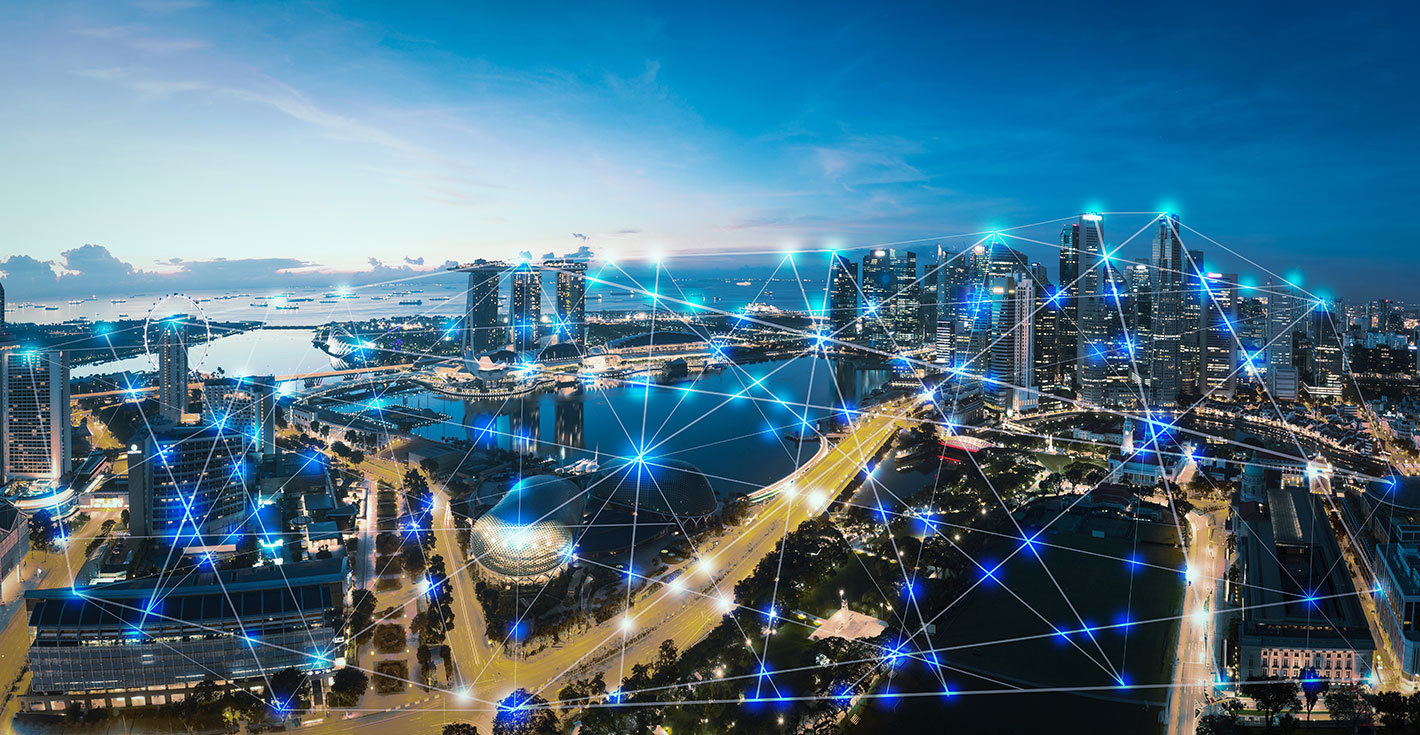
\includegraphics[width=0.8\textwidth]{media/header_main.jpg}\par\vspace{0.1cm}
    {\scshape\LARGE Mémoire de fin d’études \par}
    {\LARGE Smart grid et consommation énergétique \par}
    {\Large Comment optimiser la distribution de demain ? \par}

    \vfill

    \raggedright
    \textsc{Certin} Amélie
    \texttt{Architecture Logicielle}

    \textsc{Lairan} Alexandre
    \texttt{Architecture Logicielle}

    Maître de Mémoire : Carina Roels

    Date de soutenance : 10 mars 2020

    \vfill

    \begin{center}
      
\includegraphics[scale=0.14]{media/esgi_logo.jpg}
      \LARGE \textbf{5ESGI 2019/2020}
      
\includegraphics[scale=0.22]{media/logo_ges.png}
    \end{center}
  \end{titlepage}

  \maketitle
  \tableofcontents
  \chapter*{Résumé}

Dans l'objectif de satisfaire les attentes toujours plus importantes des politiques eco-responsables,
la recherche dans le secteur de l'énergie et la distribution de celle-ci nécessite de plus en plus d'automatisation.
Le besoin de données pour faire des prévisions réalistes, ainsi que la nécessité de micro-manager les différents noeuds
d'un réseau ont fait apparaître différents champs d'applications. Bien que les méthodes traditionnelles fonctionnent
pour de petites villes, les mégalopoles d'aujourd'hui et demain devront faire face à de nombreuses mutations.

L'énergie n'est plus distribuée de la même façon qu'il y a 20 ans, et il faut pouvoir à tout moment contrôler
le taux de saturation du réseau et l'équilibre offre/demande qui varie bien plus avec les énergies renouvelables.
De nombreuses problématiques sont a résoudre, telles que les pics de consommation la nuit, lorsque le Soleil laisse sa place
à la Lune, ou bien qu'une sécheresse assèche une STEP nécessaire au bon fonctionnement d'un pôle industriel.

Grâce à la détection des pannes, et l'amélioration des infrastructures citadines, le comportement des Hommes
s'en retrouve modifié, tout comme la 4G apporta une dimension sociale aux habitants de la ville, la 5G et les objets
connectés apporteront un nouveau canal de discussion qui permettra aux habitants de mieux comprendre la ville, et
à la ville de mieux comprendre ses habitants. Certaines villes aujourd'hui adaptent leurs offres de déplacement
collectifs en fonction des déplacements de ses habitants, demain ces offres pourront être dynamique en temps réel.

Tout ceci nous a conduit à initier des recherches sur les corrections en temps réel que l'informatique pourra
apporter, ainsi que les différentes technologies aujourd'hui mises en place pour l'utilisation des réseaux.
\chapter*{Abstract}

In order to meet the ever-increasing expectations of eco-responsible policies,
research in the energy sector and its distribution requires more and more automation.
The need for data to make realistic forecasts, as well as the need to micro-manage the different nodes
of a network have revealed different fields of application to this. Although traditional methods work
for small towns, today's and tomorrow's megacities will have to face to drastics changes.

Energy is no longer distributed in the same way as it was 20 years ago, and it must
be controled at any timethe saturation rate of the grid and the supply/demand balance,
which varies much more with renewable energies.
Many objectives have to be solved, such as peak consumption at night, when the sun leaves its place
to the moon, or a drought dries out a PHES necessary for the proper functioning of an industrial pole.

Thanks to the detection of breakdowns and the improvement of urban infrastructures, the behaviour of people
changed, just as 4G brought a social dimension to the inhabitants of the city, 5G and IoT
will provide a new channel for discussion that will allow residents to better understand the city, and
the city to better understand its inhabitants. Some cities are now adapting their travel offers
Depending on the movements of its inhabitants, tomorrow these offers will be dynamic in real time.

All this has led us to initiate research on real-time corrections that IT can make
to provide, as well as the different technologies currently in place for the use of networks.

\chapter*{Mot clefs}


\input{pre-corp/sommaire.tex}

  \chapter{État de l’art}
\section{Le dérèglement climatique}
\lipsum
\section{Augmentation des besoins en énergie}
\lipsum
\section{Guerre de l'énergie}
\lipsum
\section{Amélioration des performances informatique}
\lipsum

\chapter{Enjeux}
\section{Descriptif de la smart grid}
\lipsum

% Smart grid

% Micro grid

% Analyse des villes

\section{Villes connectées}
\lipsum
% Cette partie parlera de la partie technique de la mise en place de la smart grid
%   Ainsi que des différents problèmes que les villes actuelles ont.

\section{Connectivité et population}
\lipsum
% Cette partie parlera de la partie humaine de la connexion a la smart grid.
% ex. La 5G (6G) et les réseaux sociaux
%     Communication et report de problèmes

\chapter{Cycles énergétiques}
\section{Cycle du soleil}
\lipsum
\section{Cycle circadien humain}
\lipsum
\section{Cycles long cours}
\lipsum
% Cette partie parlera des différents cycles terrestres prenant cours sur le long terme
% ex. Courants marins - Point chaud
\section{Équilibre de la production}
\lipsum
\section{Anticipation de la consommation}
\lipsum

\chapter{Répartition des sources de production d'énergies}
% \section{}
% \section{Réutilisation des sources de chaleur}

L'emplacement des points de production sont importants dans la lutte contre le gaspillage énergétique.
Plusieurs points importants entrent en ligne de compte, comme le coût du transport de cette énergie ainsi que les pertes liées à ce mode de transport.
Peu importe la technologie utilisée, les lois de la thermodynamique rendent impossible le transport gratuit d'énergie.

\section{Perte d'énergie en chaleur}

Prenant en compte la 1ère loi de la thermodynamique, lors de toute transformation, il y a
conservation de l'énergie.
Ainsi, dans un espace clos, l'énergie ne peut varier.
Prenons pour espace le câble qui fait transiter l'énergie de la production à la consommation.

Le transport de l'énergie va transformer en chaleur une partie de celle-ci en raison
des forces de frottement des électrons sur les atomes.

Il est possible de réduire cette perte en utilisant des matériaux plus conducteurs que
d'autres, mais il n'est pas possible de l'annuler.
De plus, pour des raisons économiques, ces matériaux supraconducteurs ne peuvent être
déployés en masse du fait de leur coût, et des conditions nécessaires à leur stabilité.
Le Diborure de magnésium $MgB_2$ est un des matériaux ayant la plus haute température
critique avec 39 K (-234 C).

Aujourd'hui, la majorité des câbles électriques mondiaux sont en cuivre ou en aluminium,
on va s'intéresser plus particulièrement au cuivre qui possède le meilleur rendement.

Pour calculer la perte d'énergie dans un câble en cuivre, on peut utiliser la formule $Loss = I^2\times R$ avec $I$ pour l'intensité, exprimée en ampère, et $R$ en Ohm.
On peut exprimer les Ohms avec la formule suivante : $R = \frac{V}{I}$ avec V pour le voltage.

La formule étendue devient donc

\begin{equation} \label{loss}
  \begin{aligned}
    Loss & = \frac{I^2\times V}{I} \\
         & = I \times V
  \end{aligned}
\end{equation}

En france, on utilise la norme \texttt{NF\_C18-510} pour classer les lignes électriques

\begin{table}[h]
  \begin{tabular}{lll}
    Tension    & Courent Alternatif     \\
    Très basse & $U_n \leq 50V$         \\
    Basse      & $50V < U_n \leq 1kV$   \\
    Haute      & $1kV < U_n \leq 50kV$  \\
    Très Haute & $U_n > 50kV$
  \end{tabular}
\end{table}

% Comparons les différentes tensions pour une puissance donnée pour en obtenir.

Prenons plusieurs tensions pour une puissance donnée sur un cable d'1km de long.

Ces données vont nous donner :
\begin{itemize}
  \item Le diamètre du cable
  \item Le voltage perdu
  \item La chaleur généré
\end{itemize}



\chapter{Informatisation des infrastructures}
\section{Protocoles et Open Data}
\lipsum
% Communication entre services différents (voiture - infrastructure - éclairage - chauffage)
% Centralisation TaaS (Pilot Things)
\section{Gestion des catastrophes}
\lipsum
% Panne électrique par exemple
\section{Optimisation de la distribution énergétique}
\lipsum
\section{Cas d'étude d'une bourse de l'energie}
\lipsum

  % Avis anti-plagiat
% Charte anti-plagiat
\begin{thebibliography}{9}
  \bibitem{marine_current}
  AbuBakr S Bahaj et Luke E Myers

  \textit{Fundamentals applicable to the utilisation of marine current turbines for energy production}

  \bibitem{energy_management_smart_grids}
  Fady Y. Melhem. Optimization methods and

  energy management in ”smart grids”. Electric power.

  Université Bourgogne Franche-Comté, 2018. English.

  \bibitem{energy_demand_side}
  Hafiz Majid Hussain, Nadeem Javaid, Sohail Iqbal, Khursheed Aurangzeb et Musaed Alhussein

  \textit{An Efficient Demand Side Management System with a New Optimized Home Energy Management Controller in Smart Grid}

  \bibitem{communication_protocol}
  Sangam, Sahana \& Kulkarni, Sahana \& Jambotkar, Chaitanya. (2019).

  Smart Grid Communication Protocols. International Journal of Trend in Scientific Research and Development.

  Volume-3. 10.31142/ijtsrd21344.

  \bibitem{ev_smart_routing}
  Etesami, S. Rasoul \& Saad, Walid \& Mandayam, Narayan \& Poor, H. Vincent. (2017).

  Smart Routing of Electric Vehicles for Load Balancing in Smart Grids. 2599-2604. 10.1109/CDC.2017.8264036.

  \bibitem{nrg_consumption_scheduling}
  Stéphane Caron et George Kesidis

  Incentive-based Energy Consumption Scheduling Algorithms for the Smart Grid

  École Normale Supérieure

  The Pennsylvania State University

  \bibitem{demand_side_management}
  Peter Palensky et Dietmar Dietrich

  Demand Side Management: Demand Response, Intelligent Energy Systems, and Smart Loads

  \bibitem{stochastic_scheduling}
  Wencong Su, Jianhui Wang et Jaehyung Roh

  Stochastic Energy Scheduling in Microgrids With Intermittent Renewable Energy Resources


  \bibitem{Photovoltaic_Forecasting}
  Can Wan, Jian Zhao, Yonghua Song, CSEE, Zhao Xu, Jin Lin et Zechun Hu

  Photovoltaic and Solar Power Forecasting for Smart Grid Energy Management

  \bibitem{game_Theoretic_energy}
  Amir-Hamed Mohsenian-Rad, Vincent W. S. Wong, Juri Jatskevich, Robert Schober et Alberto Leon-Garcia

  Autonomous Demand-Side Management Based on Game-Theoretic Energy Consumption Scheduling for the Future Smart Grid

  \bibitem{Photovoltaic_life}
  V.M. Fthenakis et H.C. Kim

  Photovoltaics: Life-cycle analyses

  \bibitem{}
  Shane Duryea, Syed Islam et William Lawrance

  A Battery Management System for Stand Alone Photovoltaic Energy Systems

  School of Electrical and Computer Engineering

  \bibitem{}
  Rocco Papa

  Smart Energy in the Smart City Urban Planning for a Sustainable Future

  Romano Fistola Editors

  \bibitem{}
  ESMAP CEETI

  Planning Energy Efficient and Livable Cities

  \bibitem{}
  arcep

  L’empreinte carbone du numérique

  République française

  \bibitem{}
  Service de l’observation et des statistiques

  Chiffres clés du climat France et Monde

  République française

  \bibitem{}
  Paula Carroll et Cristina Requejo

  Smart Grid Topology Designs
\end{thebibliography}

\chapter*{Webographie}

IssyGrid
https://www.issy.com/decouvrir-issy/ville-numerique/qu-est-ce-que-la-smart-city/itineraire-d-une-ville-innovante, 03/11/2019

https://www.issy.com/issygrid, 03/11/2019

https://www.lemondedelenergie.com/issygrid-ecoquartier-smart-grid-issy/2019/05/21/, 03/11/2019

https://les-smartgrids.fr/issygrid-premier-smart-francais/, 03/11/2019

http://www.smartgrids-cre.fr/m4/index.html, 03/11/2019

https://www.issy.com/decouvrir-issy/urbanisme-grands-projets/innovation/sways-premier-batiment-d-une-nouvelle-generation, 03/11/2019

http://embix.fr/blog/portfolio/issy-grid/, 03/11/2019

https://www.banquedesterritoires.fr/issygrid-la-promesse-du-consomacteur-reste-encore-demontrer, 03/11/2019

https://www.usine-digitale.fr/article/l-exemple-d-issygrid-inspire-de-nombreux-projets-de-smart-city.N823970, 03/11/2019

https://www.somobility.fr/, 03/11/2019

https://data.issy.com/explore/?refine.theme=Transports,+D%C3%A9placements&sort=modified&disjunctive.features&disjunctive.theme&disjunctive.keyword&disjunctive.publisher, 03/11/2019

http://opentransportnet.eu/web/issy, 03/11/2019

https://opendata.hauts-de-seine.fr/explore/?refine.theme=Transport+%2F+Mobilit%C3%A9&sort=modified, 03/11/2019

https://opendata.stif.info/page/home/, 03/11/2019

https://sodigital.fr/10-ans-pour-changer-nos-mobilites/, 03/11/2019

https://www.bouygues-es.fr/liste-actualite/issygrid-premier-smart-grid-france, 03/11/2019

https://fr.calameo.com/read/000762795aa5e06a65b44, 03/11/2019

https://www.lagazettedescommunes.com/619635/lheure-du-bilan-pour-issygrid/, 03/11/2019

https://collectivites.promotelec.com/initiatives-locales/comment-issy-les-moulineaux-prepare-la-ville-de-demain-avec-le-reseau-intelligent-issygrid/, 03/11/2019

https://www.cahiers-techniques-batiment.fr/article/1a-distribution-electrique-les-smart-grids-a-l-epreuve-de-l-experimentation.23074, 09/11/2019

Toronto

http://maisouvaleweb.fr/toronto-quayside-cite-etat-numerique-etre-democratique/, 09/11/2019


https://maghrebemergent.info/la-libye-degrade-les-nappe-d-eau-souterraines-fouad-chehat-expert/
\chapter*{Annexe}
\newcommand{\hbAppendixPrefix}{A}
\renewcommand{\thefigure}{\hbAppendixPrefix\arabic{figure}}
\setcounter{figure}{0}
\begin{figure}[h]
    \centering
    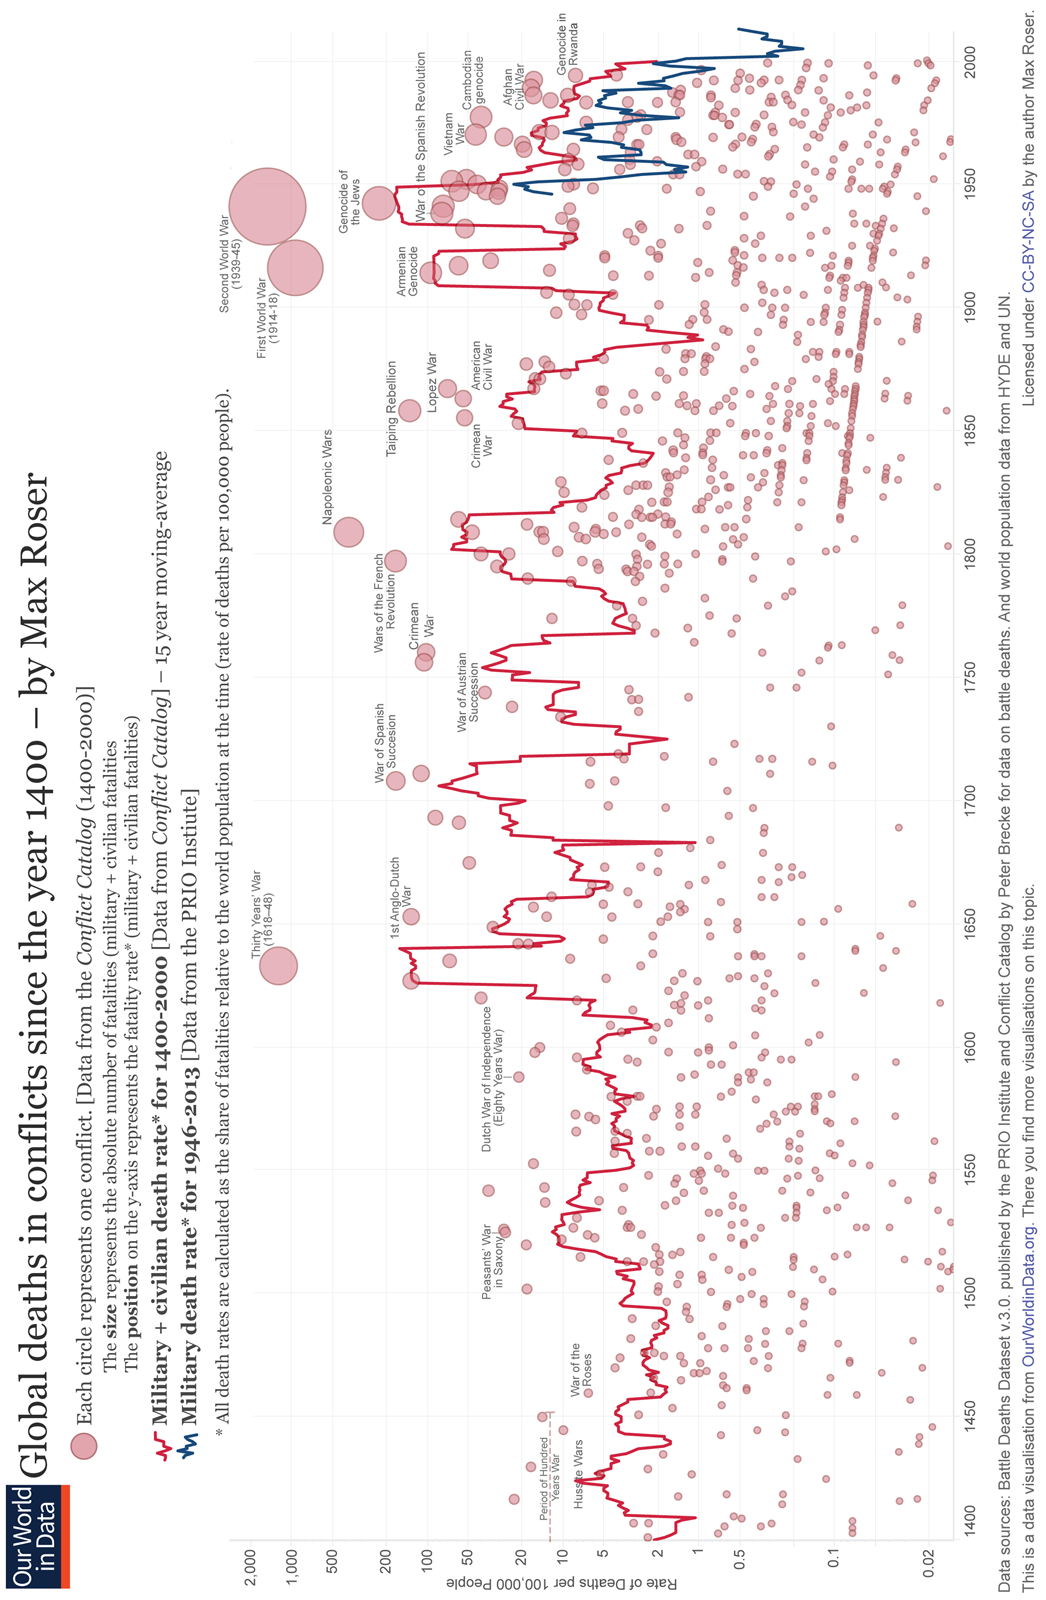
\includegraphics[scale=0.53]{media/Guerres-deces.png}
    \caption{
        Mortalité mondiale des conflits depuis 1400\newline
        \tiny{Source:
          \url{https://www.gurumed.org/2015/06/29/une-courbe-des-dcs-militaires-et-civils-depuis-lan-1400}
        }
    }
  \end{figure}


\section*{Interview}
\textbf{Alexandre C.} :
L'objectif de ce projet était d’expérimenter la connexion d’un morceau de ville à internet.
Il y avait trois défis : la collecte de données par l’installation de capteurs,
la récupération de données sur internet et le développement d’outils logiciels capables de traiter ces données.
Ça a pris la durée sur tout le long du projet. Tout d’abord dans le quartier des affaires,
là où sont implantés la majeur partie des entreprises d'Issy-les-Moulineaux – dont Bouygues Immobilier.
Puis le projet a été étendu aux nouveaux quartiers résidentiels dans un second temps.

\textbf{Quel a été l’impact de la smart Grid sur les entreprises présentes dans la Smart Grid ?}

\textbf{Alexandre C.} :
Ça n’a pas réellement changé leur façon de vivre, mais leur confort s'est amélioré.
Prenons l'exemple du siège de Bouygues Immobilier, dans le bâtiment Galéo.
Il y avait peu de visibilité sur ses consommations énergétiques
et ses factures sans instrumentation pour mesurer ses performances énergétiques.
Le projet a permis de mettre en place les capteurs nécessaires pour remédier à ce problème.
Ils connaissent maintenant leur consommation et l’état de santé de leur bâtiment en temps réel.
Ils ont repéré pas mal de dysfonctionnements dans leur consommation.
Notamment sur le plan thermique, avec des température dont le réglage était incorrecte
et des fuites de chaleur aux niveaux de vannes qui devraient se fermer automatiquement.
Le confort pour les occupants n’était pas forcément assuré.
D'autres capteurs pour mesurer la qualité de l’air ont montré qu'elle se dégradait dans les salles de réunion après un certain temps.
L’objectif principal de la Smart Grid pour ce bâtiment était de pouvoir évaluer la performance
et le confort afin de pouvoir prendre les décisions pour corriger ces dysfonctionnements.
On navigue à l’aveugle sans ces outils logiciels.
Il est compliqué d’estimer le véritable gain monétaire, ou de performance,

\textbf{Comment étaient gréffés les objets connectés au réseau ?}

\textbf{Alexandre C.} :
Alors il y a eu plusieurs types de capteurs.

Tout d’abord sur les bâtiments du tertiaire.
Aujourd’hui l’instrumentation est faite de manière systématique sur les bâtiments neufs.
Ils sont équipés de capteurs qui ne discutent pas directement sur Internet,
mais qui sont reliés entre eux au sein d’un réseau filaire avec des protocoles de communication
tels que Modbus, BACnet, qui permettent de communiquer via des câbles ethernet ou Modbus
et de partager leurs informations entre eux.
Derrière il y a des outils logiciels, communément appelés GPB (Google Protocol Buffers) qui accèdent à ce réseau
pour interfacer en temps réel les données de tous les capteurs.
C'est le GPB qui fait la connexion à Internet pour rendre visibles ces données depuis l'extérieur.
La mise en place du réseau a été livré en même temps que les bâtiments.
Mais pour avoir accès à l’information par Internet il a fallu quelques travaux en plus.

Le fonctionnement est différent dans les bâtiments d'habitation.
Dans chacun des 600 logements, il y a eu un gros compteur installé
auquel est relié tout un réseau de capteurs capables de lui transmettre l’information en filaire :
température, consommation de chauffage, consommation électrique\dots
Le compteur, lui est connecté directement à Internet.

La Smart Grid récupère aussi des informations via des objets connectés dans la ville,
notamment sur la Gare SNCF, Val-de-Seine (RER C).
Il y a un objet connecté posé directement sur le compteur ENEDIS pour mesurer la consommation électrique via un réseau longue porté, LoRa.
Il s’agit d’un réseau déployé par Bouygues Telecom qui couvre tout le territoire français en passant par les ondes radio.
Le maillage en France est de l’ordre du kilomètre.
Ces objets connectés compatibles LoRa peuvent donc communiquer en utilisant ces antennes là.
La donnée est ensuite stockée sur les serveurs de Bouygues Telecom.
L’avantage est qu’il n’y a pas de câble, ce qui est très pratique pour l’installation.

Les réseaux électriques et thermiques sont gérés par ENEDIS.
Ils équipent les appartements récents des compteurs Linky leur permettant de récupérer à distance les données de consommation.
Les données journalières sont automatiquement enregistrées sur les serveurs ENEDIS.
Avec l’accord du consommateurs, il peut faire un enregistrement toutes les 30 minutes.
N’importe quel acteur qui dispose du consentement de l’abonné au réseau peut récupérer la donnée de consommation énergétique auprès de ENEDIS.
Dans le cadre d’un projet urbain par exemple.
Mais il n'est pas possible de communiquer directement avec les compteurs.
Le rôle d'Embix était donc d'assurer la collecte de données et le développement des interfaces pour voir ces données.

\textbf{Y avait-il d'autres capteurs en ville ? Pour gérer le trafic au niveau des feux rouges par exemple ?}

\textbf{Alexandre C.} :
Dans une rue du le quartier d’affaire, il y a des capteurs au niveau de l’éclairage public.
On récupère la donnée à distance pour savoir si un éclairage est allumé ou non.
L’échange est bidirectionnel, on peut envoyer un signal au luminaire pour qu’il s’éteigne par exemple.
Il y a aussi des capteurs de présence pour les piétons et véhicules, pour ajuster l’éclairage public et n’éclaire qu’en cas de besoin.
C’est à dire lorsqu’il y a un piéton ou véhicule en approche.
L’éclairage n’est pas totalement éteint, on ajuste la puissance de l’éclairage de la rue.
S’il n’y a personne, on réduit l’intensité lumineuse.
On a pu diviser par 2 la consommation de l’éclairage public avec ce système.
Ça n’a pas été compliqué à mettre en oeuvre et le résultat était immédiat.
Il y a eu des sujets autour de ces luminaires pour en faire des points relais wifi, mais ce projet n’a pas abouti.
L'exemple que vous avez cité – la gestion du trafic par les feux tricolores) n’a pas été implémenté dans IssyGrid.
Il y a des villes plus connectées que d’autres, Montpellier, Dijon, Angers, qui investissent beaucoup dans ce domaine.
Ils proposent par exemple des données permettant de trouver des places de parking disponibles.
Des capteurs de présence et de géolocalisation relèvent les places de parkings disponibles
et permettent d’alimenter des applications pour relayer l’information à la population avec un mapping des places de parkings.
Il me semble qu’il y a des applications de ce type là à Nice ou Lyon.
Mais on est plus dans de la Smart City que de la Smart Grid.
L’utilisation de ces données là dans une Smart Grid a pour but l’économie d'énergie :
électricité, chaleur, consommation d’eau également\dots

\textbf{Est-ce que la Smart Grid a permis à la ville d’avoir un mix énergétique un peu plus vert ?}

\textbf{Alexandre C.} :
C’est une sacrée question, et vous n’aurez pas la même réponse selon l’interlocuteur.
Il y a plusieurs périmètres.
D’une part à l’échelle du territoire international, il y a un besoin d’équilibrer la consommation d’électricité et sa production.
La personne morale responsable de ce niveau est RTE (Réseau de Transport de l’Electricité), une entreprise française semi-publique.
Sa mission est d’équilibrer production et consommation grâce à de l’analyse prédictive de la consommation en électricité
de l’heure suivante à 1\% près sur le territoire français.
Elle s’appuie sur les productions des centrales nucléaire, mais également de plus en plus de production renouvelables : photovoltaïque, éolien\dots
Mais les énergies renouvelables posent un défi supplémentaire puisque leur production est intermittente,
à cause de la météo notamment, contrairement à la centrale nucléaire où la production est à la demande.
Une Smart Grid à l’échelle nationale est capable de prédire ces données météo pour adapter la distribution en temps réel.
Il y a quelque chose de très bien développé en France qui est l’effacement.
Les gros consommateurs d'électricité comme des industriels se mettent d’accord entre eux et avec le réseau
pour ne plus consommer pendant un laps de temps.
Par exemple, RTE détermine que la consommation en France à 19h va être très élevée
et qu’elle n’est pas capable de répondre à la forte demande considérant son nombre d’unités de production.
Elle va donc demander à de gros consommateurs d’arrêter de consommer pendant une courte période.
La Smart Grid permettrait donc de faire ces analyses et ses demandes d’effacement de façon automatique.
Plus on utilise d’énergie renouvelable, plus on a besoin de recourir à cette politique d’effacement
car la production est moins prévisible et nous deviendrons dépendants des ces logiciels là.
A l'échelle de la collectivité, les volumes de production installés dans les communes
n’est pas encore assez important la plupart du temps pour poser problème.
Dans le cas d’une petite ville qui aurait fait le choix de grand parcs d’énergies vertes,
il faudrait construire le projet avec ENEDIS qu’il n’y pas de soucis particulier dans le réseau.
A ce jour, je n’ai pas vu de genre de “réel” Smart Grid.
Mais je l’ai vu sur des espaces privés.
Nous avions un projet sur le site du siège social de Bouygues Construction du coté de Saint-Quentin-en-Yvelines.
C’est une petite ville avec entre 1 000 et 5 000 personnes qui travaillent.
C’est un territoire privé, donc il est possible de réaliser des optimisations énergétiques à cette échelle.
Sur un territoire public, les optimisations de réseau sont déjà faite par RTE et ENEDIS,
donc il n’y a pas trop d'intérêt à optimiser une deuxièmes fois la consommation.
C’est déjà de leur responsabilité et par extension celle de l’État.

\textbf{Ce n’est donc pas à la Smart Grid de gérer l'équilibre, son but est d’informer RTE qu’un équilibre peut être rompu ?}

\textbf{Alexandre C.} :
Oui c’est un peu ça. Smart Grid est un mot qui peut désigner beaucoup de choses.
Mais à partir du moment où on manipule de l’information on est déjà en train de faire du Smart Grid.
Le deuxième avantage de la Smart Grid est de pouvoir mapper le réseau et détecter les dysfonctionnements en temps réel
quand une alimentation électrique est coupée pour intervenir immédiatement.

\textbf{J’ai vu qu’il y avait pas mal de nouvelle technologies qui venaient de voir le jour justement pour rééquilibrer les périodes creuses.
Des petites unités d’hydrogènes qui se mettaient proches des énergies intermittentes.}

\textbf{Alexandre C.} :
On peut parler du stockage un peu de manière générale.
C’est une manière différente de contribuer à l’équilibre entre offre et demande.
Si on a trop de production photovoltaïque, on peut stocker sous sous forme de batterie,
soit sous forme d’hydrogène, ou d’une autre manière l'énergie excédentaire pour la restituer plus tard.
Les grosses centrales photovoltaïques sont couplées avec du stockage afin de pallier à cette intermittence.
Les systèmes de stockages peuvent contrebalancer les déséquilibres dus à la météo afin de lisser la production et mieux prévoir la quantité produite.
Les batteries permettent aussi de faire de l’effacement.
On stocke au moment où l’électricité est pas chère et la libérer lorsque le réseau en a besoin, au moment où le coût de l’électricité est plus élevé.
Avec l'excédent de production on peut aussi fabriquer de l’hydrogène.
Soit on utilise ensuite l’hydrogène tel quel et le revendre à des industriels, par exemple dans de stations service de véhicules à hydrogène.
On peut aussi restituer l’électricité à partir de l’hydrogène et s’en servir comme d’une batterie. Tout cela est encore expérimental,
on n’a pas encore trouvé de véritable modèle économique. Et les coûts sont encore trop élevés pour que ça puisse fonctionner à grande échelle.


\textbf{Comment se sont rassemblés tous les acteurs du projet ? Y-a-t'il eu un appel d'offre ?}

\textbf{Alexandre C.} :
L’impulsion initiale a été lancée par Bouygues et la ville, mais le projet a été lancé par tous les partenaires.
Ce projet est particulier dans le sens où il a été financé par les partenaires du projet.
Les entreprises du consortium ont toutes investi la somme de 250 000€ – si je ne me trompe pas.
Bouygues Energies \& Services, Bouygues Immobilier, General Electric, EDF, ENEDIS, Microsoft, Objenious, Schneider Electric, Sopra Steria et Total.
Les plus gros acteurs industriels ont décidé collectivement d’expérimenter là dessus pour voir quels seraient les gains réalisés dans ce domaine.
Pour se rendre compte des difficultés qui pourraient être rencontrées notamment en terme de collecte de données.
Il n’y a pas eu d’appel d’offre, de sélection pour créer ce projet là.
Ni de subvention particulière, c’est de la R\&D.
Derrière il y avait des partenaires du projet comme Embix ne faisant pas partie du consortium car ils n'avaient pas fait d’apport budgétaire.
Le pot commun a permis de financer les travaux. Il a été utilisé pour faire travailler des entreprises comme la nôtre.
Embix a été créé en 2011 à l’occasion de ce projet par des membres du consortium,
les trois actionnaires de l’époque : Bouygues Immobilier, Bouygues Energie et Service, et General Électric,
anciennement Alstom Grid – ils ont été rachetés depuis.

\textbf{Embix a donc eu d'autres projet après IssyGrid ?}

\textbf{Alexandre C.} :
Aujourd’hui, General Electric n’est plus dans notre actionnariat. Il ne reste plus que Bouygues Immobilier, et Bouygues Électrique et Service.
On travaille sur une quarantaine d'autres projets – à des stades de développement divers – maintenant que IssyGrid est terminé.
On a pas mal de projets à Paris, plusieurs à Lyon aussi, quelques villes en France, on a un projet au Maroc, un autre sur l’Ile Maurice\dots
On commence à avoir pas mal de choses en France et à l’international en somme.
Chacune des villes a sa problématique, mais on retrouve un même besoin partout qui est de suivre la consommation énergétique.
Ils renouvellent le parc immobilier en créant de nouveaux quartiers et en promettant des quartiers éco-responsables.
Mais quand on mesure – si on mesure – on se rend compte que les performances énergétiques ne répondent pas aux critères énoncés initialement.
Notre rôle est d’instrumenter le quartier pour récupérer de la donnée, regarder la performance et la comparer avec ce qui était prévu.
Puis apporter les corrections nécessaires pour que le quartier fonctionne correctement.
Comme je le disais tout à l’heure, chacun a sa définition de la Smart Grid.
La seule chose en commun entre toutes ces définitions est la notion de préservation de l’énergie et la collecte des données.
Ce qu’on en fait ensuite dépend de celui qui la manipule, chacun apporte sa pierre à l’édifice.

\textbf{Vous êtes-vous inspirés d’autres projets de Smart Grid lors de l’instruction du projet d’IssyGrid ?}

\textbf{Alexandre C.} :
Les personnes qui intervenaient dans le consortium avaient par le passé participé à d’autres projets.
En France pas vraiment, puisque IssyGrid est une première.
Il y a eu des projets démonstrateurs un peu avant, sur des périmètres contrôlés.
Il y a eu un projet qui a fait un peu parler de lui, Nice Grid.
L’inspiration du projet a pu venir des États-Unis et d’Angleterre.
Mais le fonctionnement est là-bas, les réseaux de transport et de distribution sont des acteurs privés.
Ils se permettent d'aller un peu plus loin dans l’optimisation énergétique et proposent des choses plus innovantes.
L’un des freins à la Smart Grid en France, puisque c’est public,
les infrastructures sont sur-dimensionnés pour éviter toute coupure électriques – ou presque.
Pour que le réseau ne tombe pas chez nos voisins anglais ou allemand, ils ont besoin de plus de surveillance.
Les Smart Grids sont donc plus développées dans ces pays là.
Les choses tendent à évoluer en France car l’État commence à être plus regardant sur les dépenses de ENEDIS et RTE,
et demande de moins surdimensionner et de mieux équilibrer offre et demande.
On rentre dans des discussions assez politiques du fait que le réseau soit public malheureusement.
Le fonctionnement du réseau en France impacte les projets de Smart Grid.
C’est donc un frein au développement de l’activité en France et je pense que mon avis est partagé par les acteurs du secteur.
Pardon, je crois que je me suis écarté de la question.
Nous avons surtout appris au cours du projet, il a quand même duré 8 ans !
Ce genre de projet démonstrateur et R\&D dure d'ordinaire 3 ou 4 ans.
Ce sont surtout les autres projets qui se sont inspirés d’IssyGrid et non l’inverse.
Il a beaucoup rayonné dans le monde. On a encore aujourd’hui des délégations chinoises ou japonaises.


\textbf{Quels enseignements avez vous pu tiré de ce projet au cours de ces 8 années, et quelles étaient les quick win
– les actions mises en place avec peu d’effort mais à forte valeur ajoutée ?}

\textbf{Alexandre C.} :
La collecte de données a été complexe en l’absence de standardisation.
Les capteurs utilisés sur les bâtiments et par chaque fournisseurs sont différents et communiquent par des protocoles tout aussi différents.
Nous avons dû apprendre à communiquer avec une quinzaine de protocoles différents afin d’agglomérer l’information en un endroit
et de la rendre accessible via une interface.
C’est plus rapide à apprendre qu’une langue vivante mais parfois dans certains cas ça reste un vrai défi.
Il n’y avait pas vraiment de projets existants de cette envergure : 600 logements, 15 bâtiments tertiaire, une gare…
Ce qui représente beaucoup de types de données différentes.
Un de nos quicks win est sans doute l’éclairage public. Plusieurs villes font ça maintenant.
Il y a aussi eu quelques essais de stockage de froid dans un grand bâtiment.
Et je parle d’une grande tour, comme ce qu’on pourrait avoir à la Défense – je ne pourrais pas vous dire la taille exacte.
Cette grande tour a une consommation d’énergie conséquente, notamment l’été en pour faire tourner la climatisation.
La nuit – durant les heures creuses – on va volontairement consommer plus d’électricité pour fabriquer de la glace.
Et lorsqu’il y a des problèmes de chaleur vers 14h en semaine, plutôt que de faire fonctionner la climatisation,
on va laisser fondre ce bloc de glace pour produire de l’électricité. Ce bloc de glace est en fait utilisé comme une batterie.
Ce n’est pas très cher à mettre en place – à l’échelle du bâtiment – et à utiliser.
C’est intéressant puisque ces problèmes de climatisation et de consommation est un véritable sujet à la Défense,
et on pourrait réduire leur consommation en les équipant de ce système, et donc éviter de surdimensionner le réseau électrique.
Indépendamment du réseau, il y a un gain économique à ce stockage.

\textbf{Quelles seraient les différences entre un projet Smart Grid créé aujourd’hui et un projet dans 5 ans ?}

\textbf{Alexandre C.} :
Question difficile. Tout d'abord le projet ne serait pas initié par les mêmes personnes.
Au début d’IssyGrid, il n’y avait que peu de projets et peu d’acteurs. Et les projets consistaient surtout en de la R\&D.
Aujourd’hui, les quartiers de ce types seraient initiés par les promoteurs immobiliers.
Ils profitent de la construction de nouveaux quartiers pour bénéficier de ces technologies.
Une autre différence est qu’avant on mettait beaucoup l’accent sur la recherche de l’équilibre offre-demande avec de l’intelligence artificielle,
des algorithmes d’optimisation compliqués.
Il faudrait vraiment que le réseau locale présente des particularités pour mettre en place tous ces procédés.
Une station de ski par exemple, qui n’est alimenté que par une source.
Il y aurait un risque de coupure en électricité si la ville consomme trop.
Aujourd’hui on chercherait plutôt la tenue de la performance.
On s’est rendu compte qu’en instrumentant pour récupérer de la données que nos systèmes énergétiques
ne fonctionnent pas bien en France, car personne ne surveille.
Une Smart Grid s’attache a établir des objectifs de performance et apporter une solution technique pour suivre cette performance.

Nous remercions M. Alexandre Capelle d'avoir pris le temps de répondre à nos questions avec autant de détails.

\end{document}
